%Paulin VIOLETTE
%Si t'as pas bossé sur l'interface utilisateur t'y touche pas.
%Sauf si la personne dont le nom est écris en haut te dis d'y toucher.
\chapter{Interface Utilisateur}

\section{Présentation}

%Mettre l'image de ma super interface grave stylé
\begin{figure}[h]
  \centering
  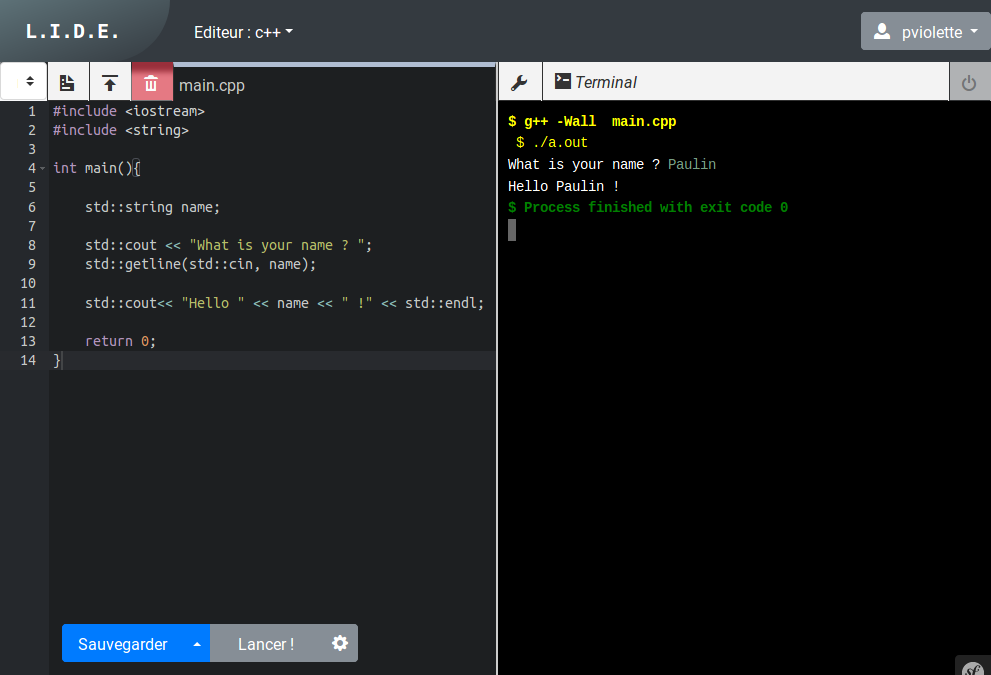
\includegraphics[width=0.8\textwidth]{./frontend/example1.png}
  \caption{Interface utilisateur en utilisation}
  \label{}
\end{figure}

Blabla fonctionnement de l'interface en générale

\section{Outils utilisés}

%Blabla HTML/CSS/JS, generateur de template twig, Framework bootstrap
%Utilisation de jquery
%Editeur ace
%SweetAlert2 pour les alertes trop swag
%JQConsole vite zef parceque c'est valou qui l'a fait

\subsection{Organisation des templates TWIG}

\section{Environnement de Développement}

\subsection{Gestions des langages}
Blabla DB changement de langage

\subsection{Éditeur de texte}
Tres court parce que y'a pas grand chose à dire

\subsection{Personnalisation}

\begin{figure}
\centering
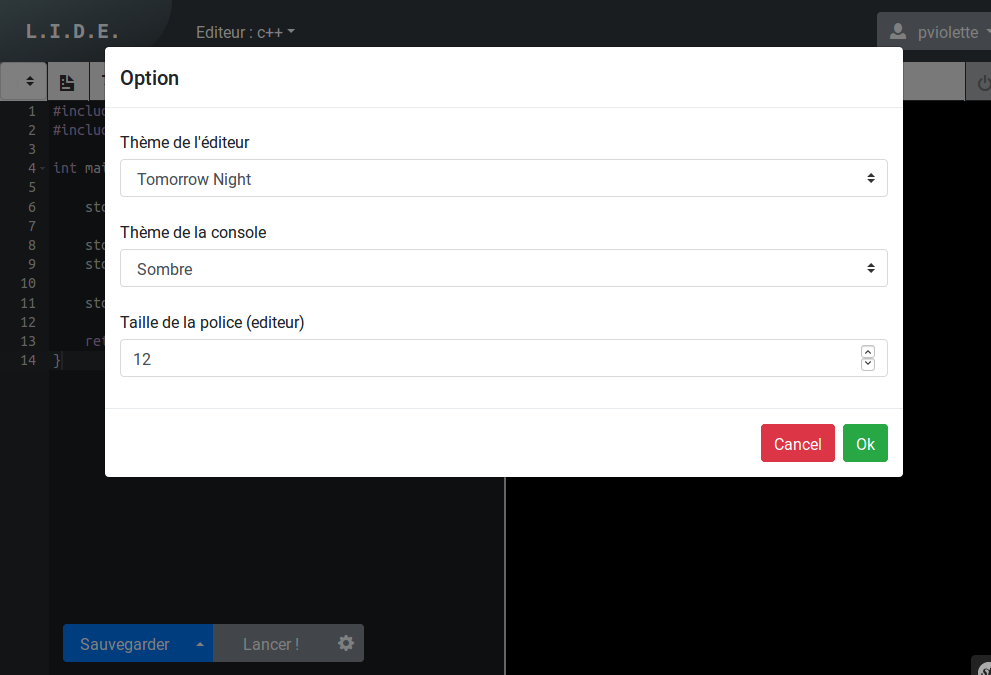
\includegraphics[width=0.8\textwidth]{./frontend/example_personnalisation.png}
\caption{Formulaire permettant la personnalisation de l'interface}
\end{figure}

\subsection{Gestions des fichiers}
Blabla full JS import export trop bien cool il est minuit j'écris nimp

\section{Compilation et exécution du code écris}
Ce titre pu

\subsection{Formulaire}

SS de mon formulaire trop swag

\subsection{Terminal}

Vas y valou tu 'écrira ça
